\documentclass{article}
\usepackage[utf8]{inputenc}
\usepackage{minted}
\usepackage{graphicx}
\usepackage{hyperref}
\usepackage[dvipsnames]{xcolor}


\title{fixation tagconnect et ouverture boitier}
\author{cmonaton }
\date{October 2019}

\begin{document}

\maketitle

\section{Introduction}

Voici des méthodes pour maintenir connecté le tag-connect à la carte pour faciliter l'utilisation ainsi que la méthode la plus simple pour ouvrir l'écran du boitier pour ne pas le casser.


\section{Fixation tag-connect}

\begin{figure}[H]
\begin{center}
\advance\leftskip-3cm
\advance\rightskip-3cm
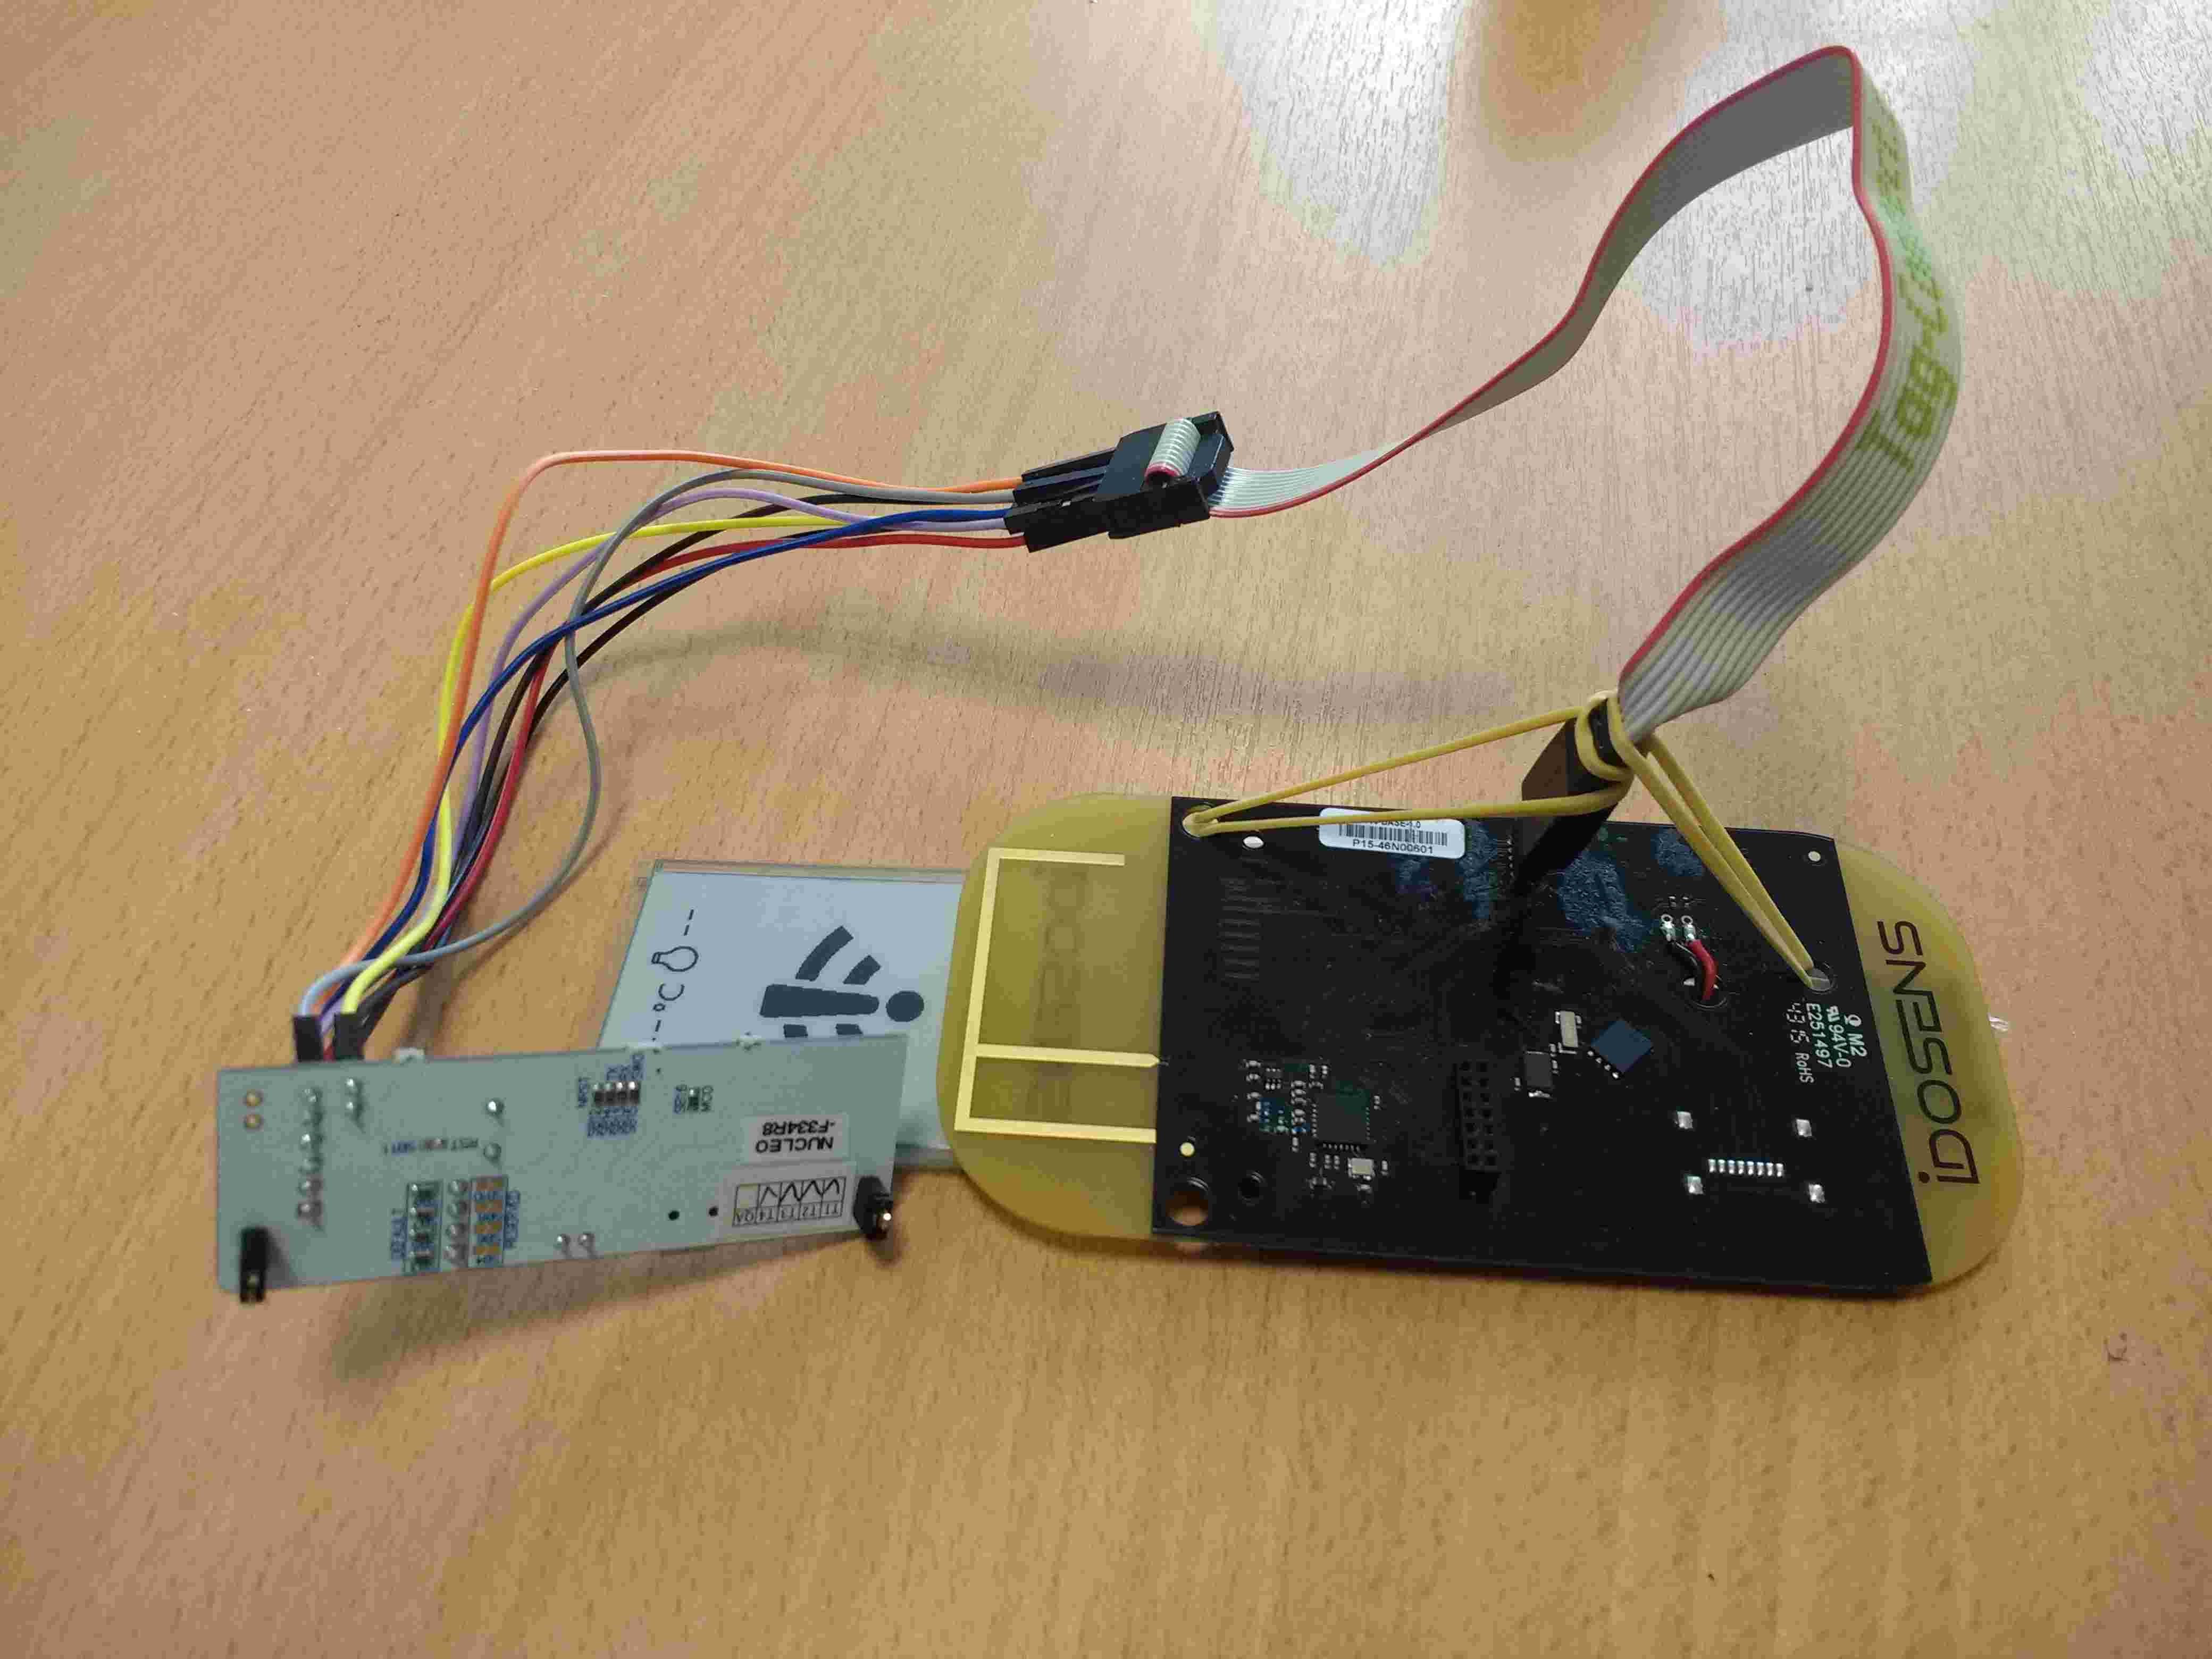
\includegraphics[keepaspectratio=true,scale=0.1]{fixation_tagconnectface.jpg}
\label{visina8}
\end{center}\end{figure}

\begin{figure}[H]
\begin{center}
\advance\leftskip-3cm
\advance\rightskip-3cm
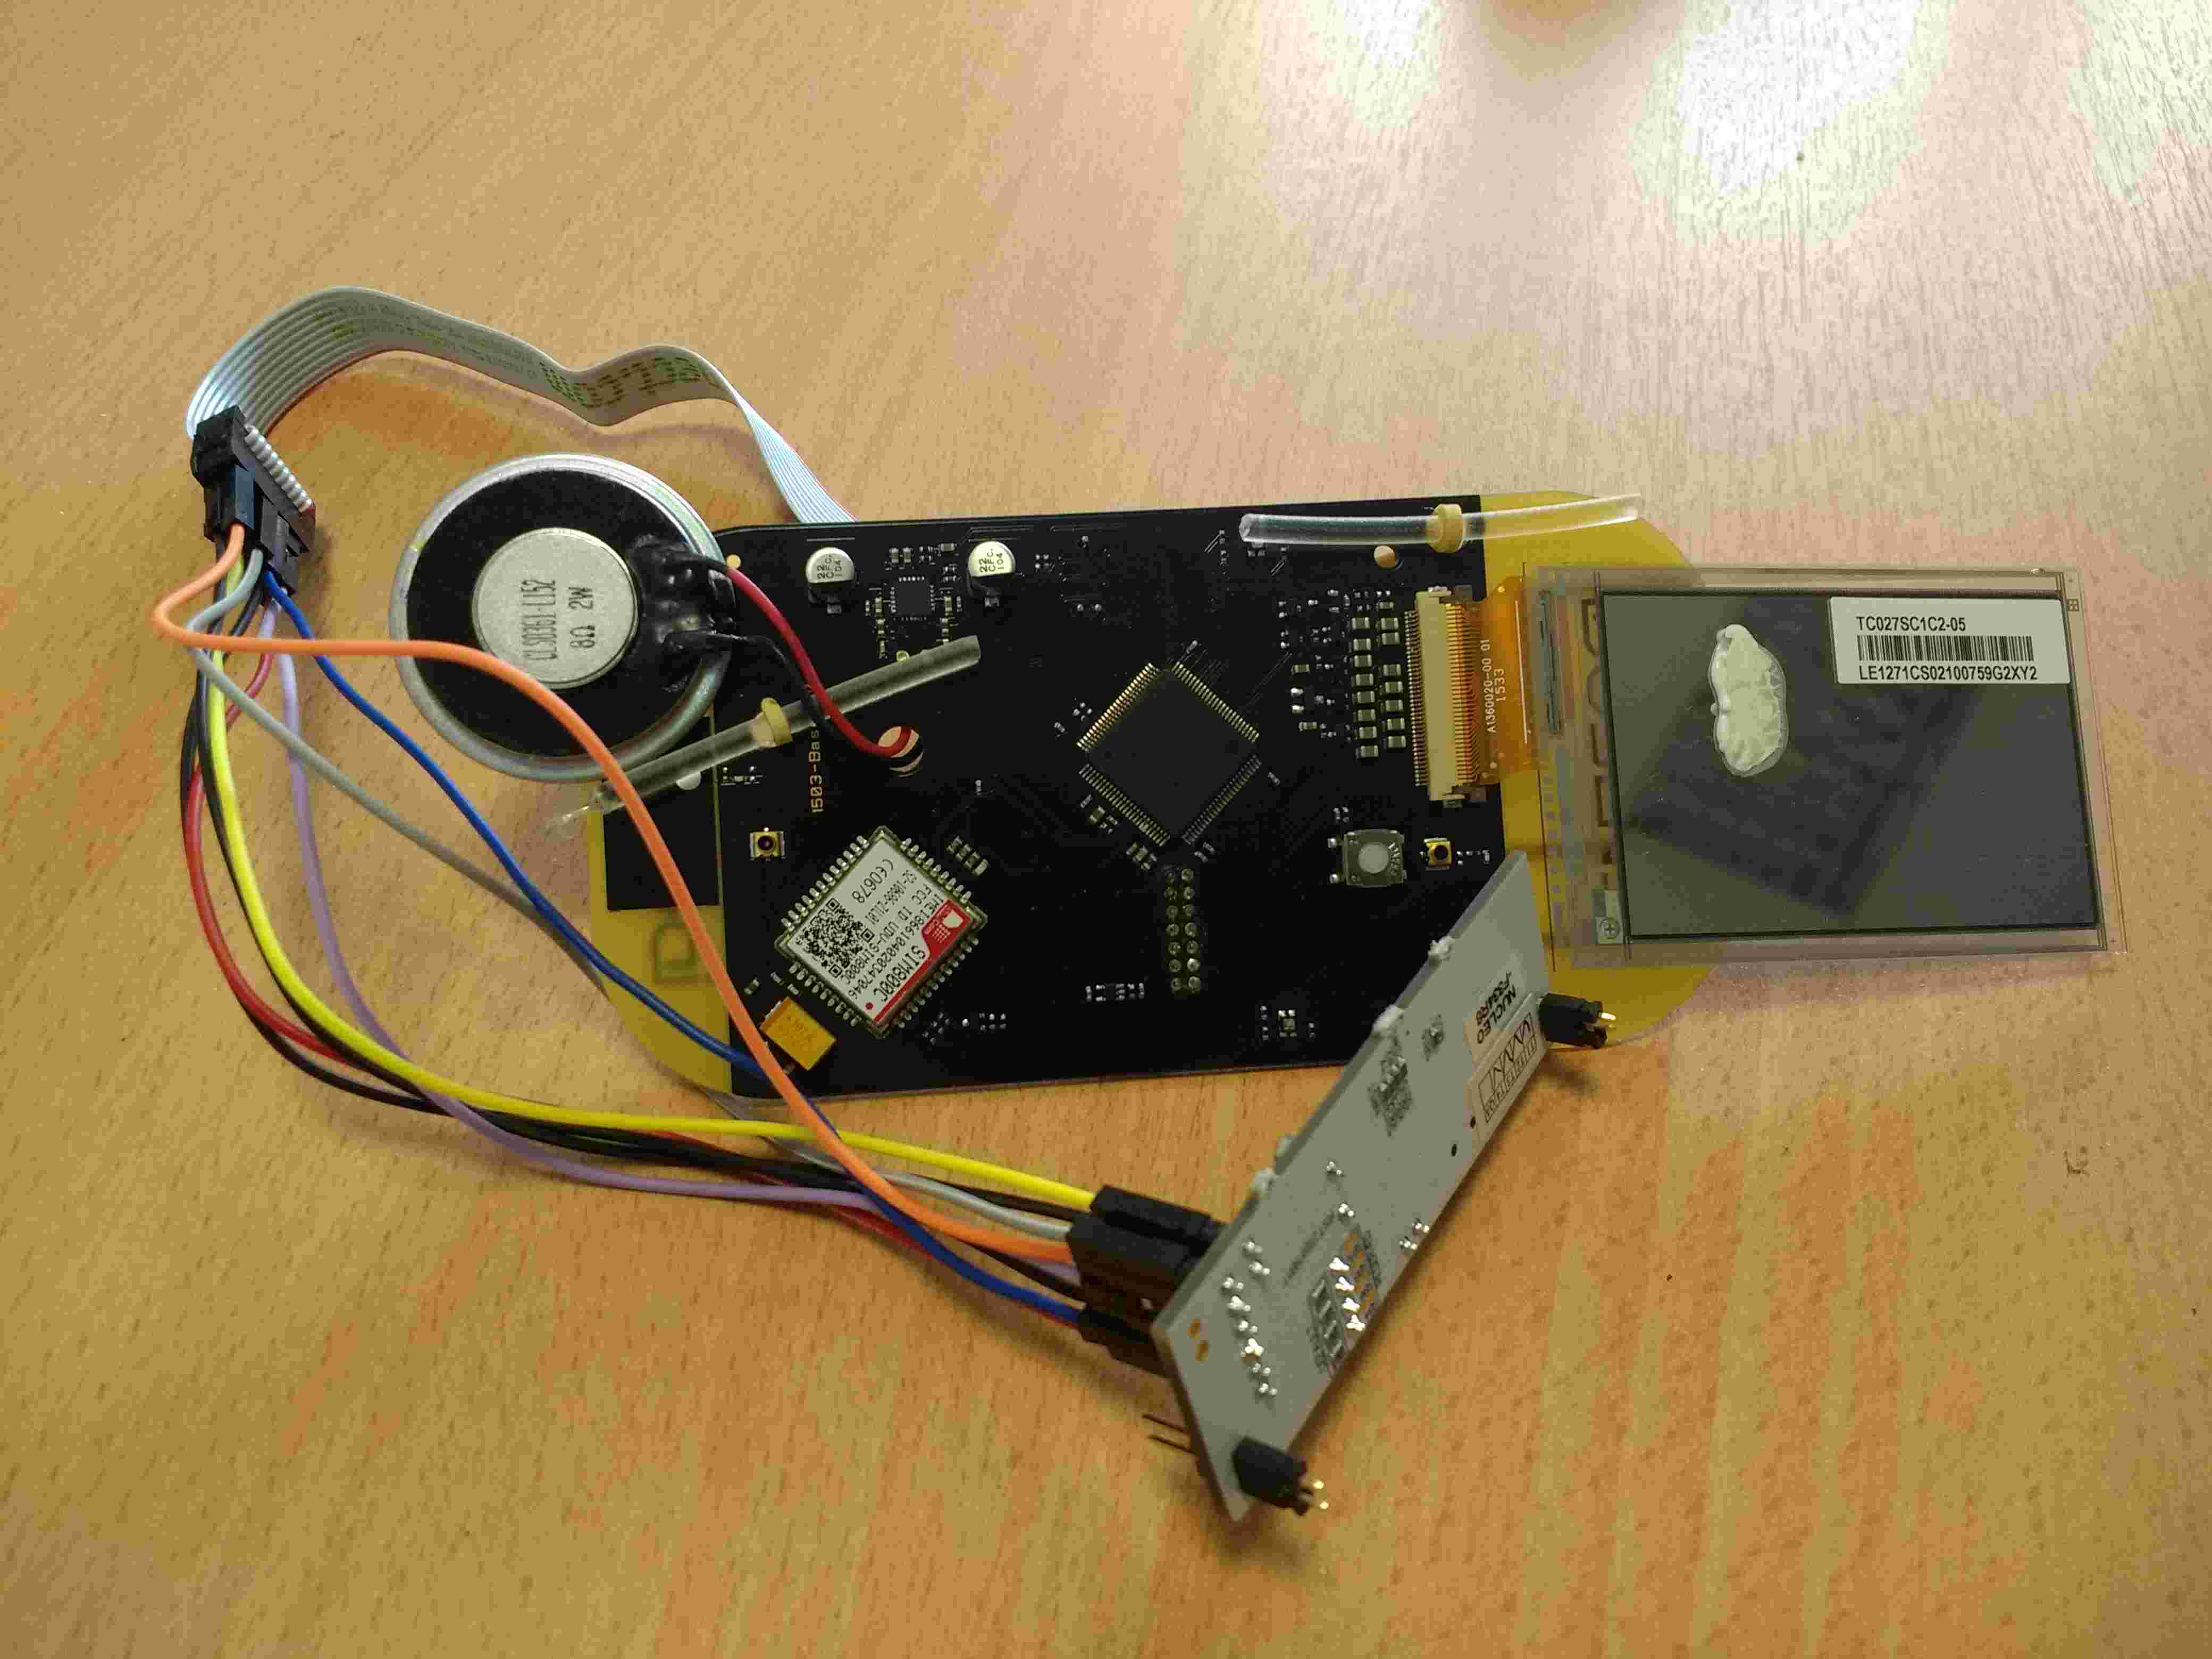
\includegraphics[keepaspectratio=true,scale=0.1]{fixation_tag-connectdos.jpg}
\label{visina8}
\end{center}\end{figure}

\begin{figure}[H]
\begin{center}
\advance\leftskip-3cm
\advance\rightskip-3cm
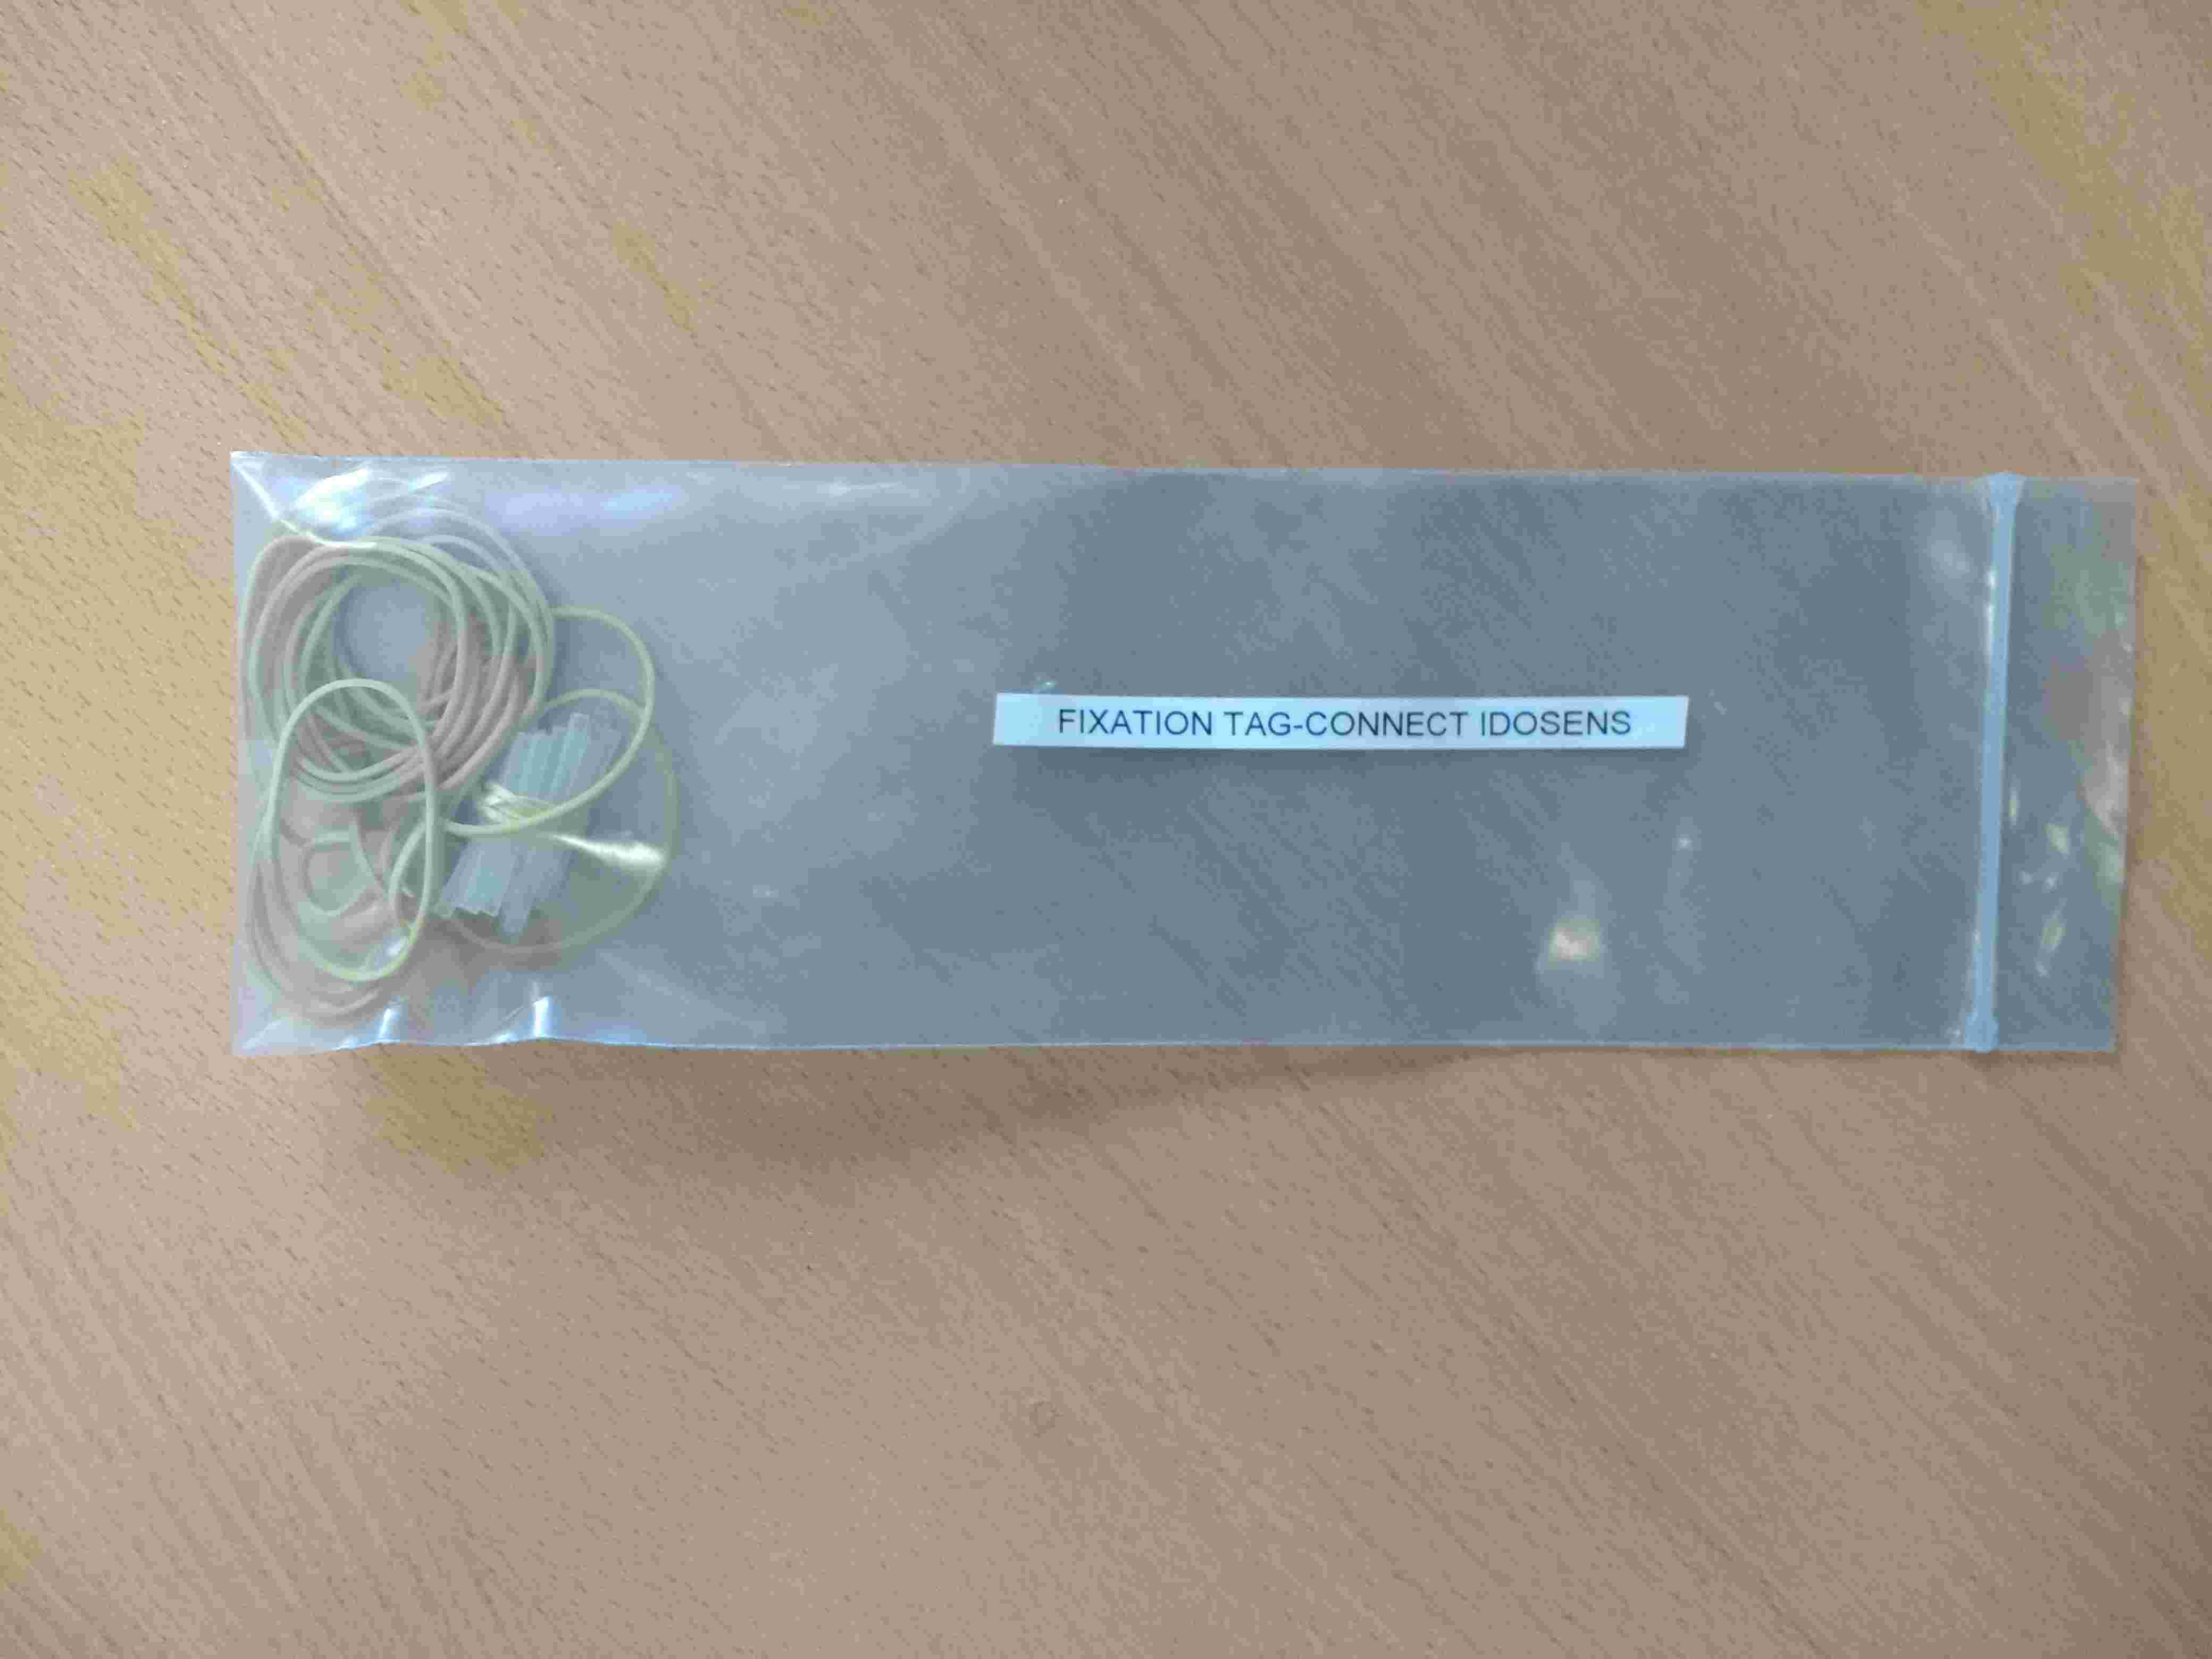
\includegraphics[keepaspectratio=true,scale=0.1]{fixation_tagconnect_idosens.jpg}
\label{visina8}
\end{center}\end{figure}

\section{Ouverture/fermeture écran boîtier}

\begin{figure}[H]
\begin{center}
\advance\leftskip-3cm
\advance\rightskip-3cm
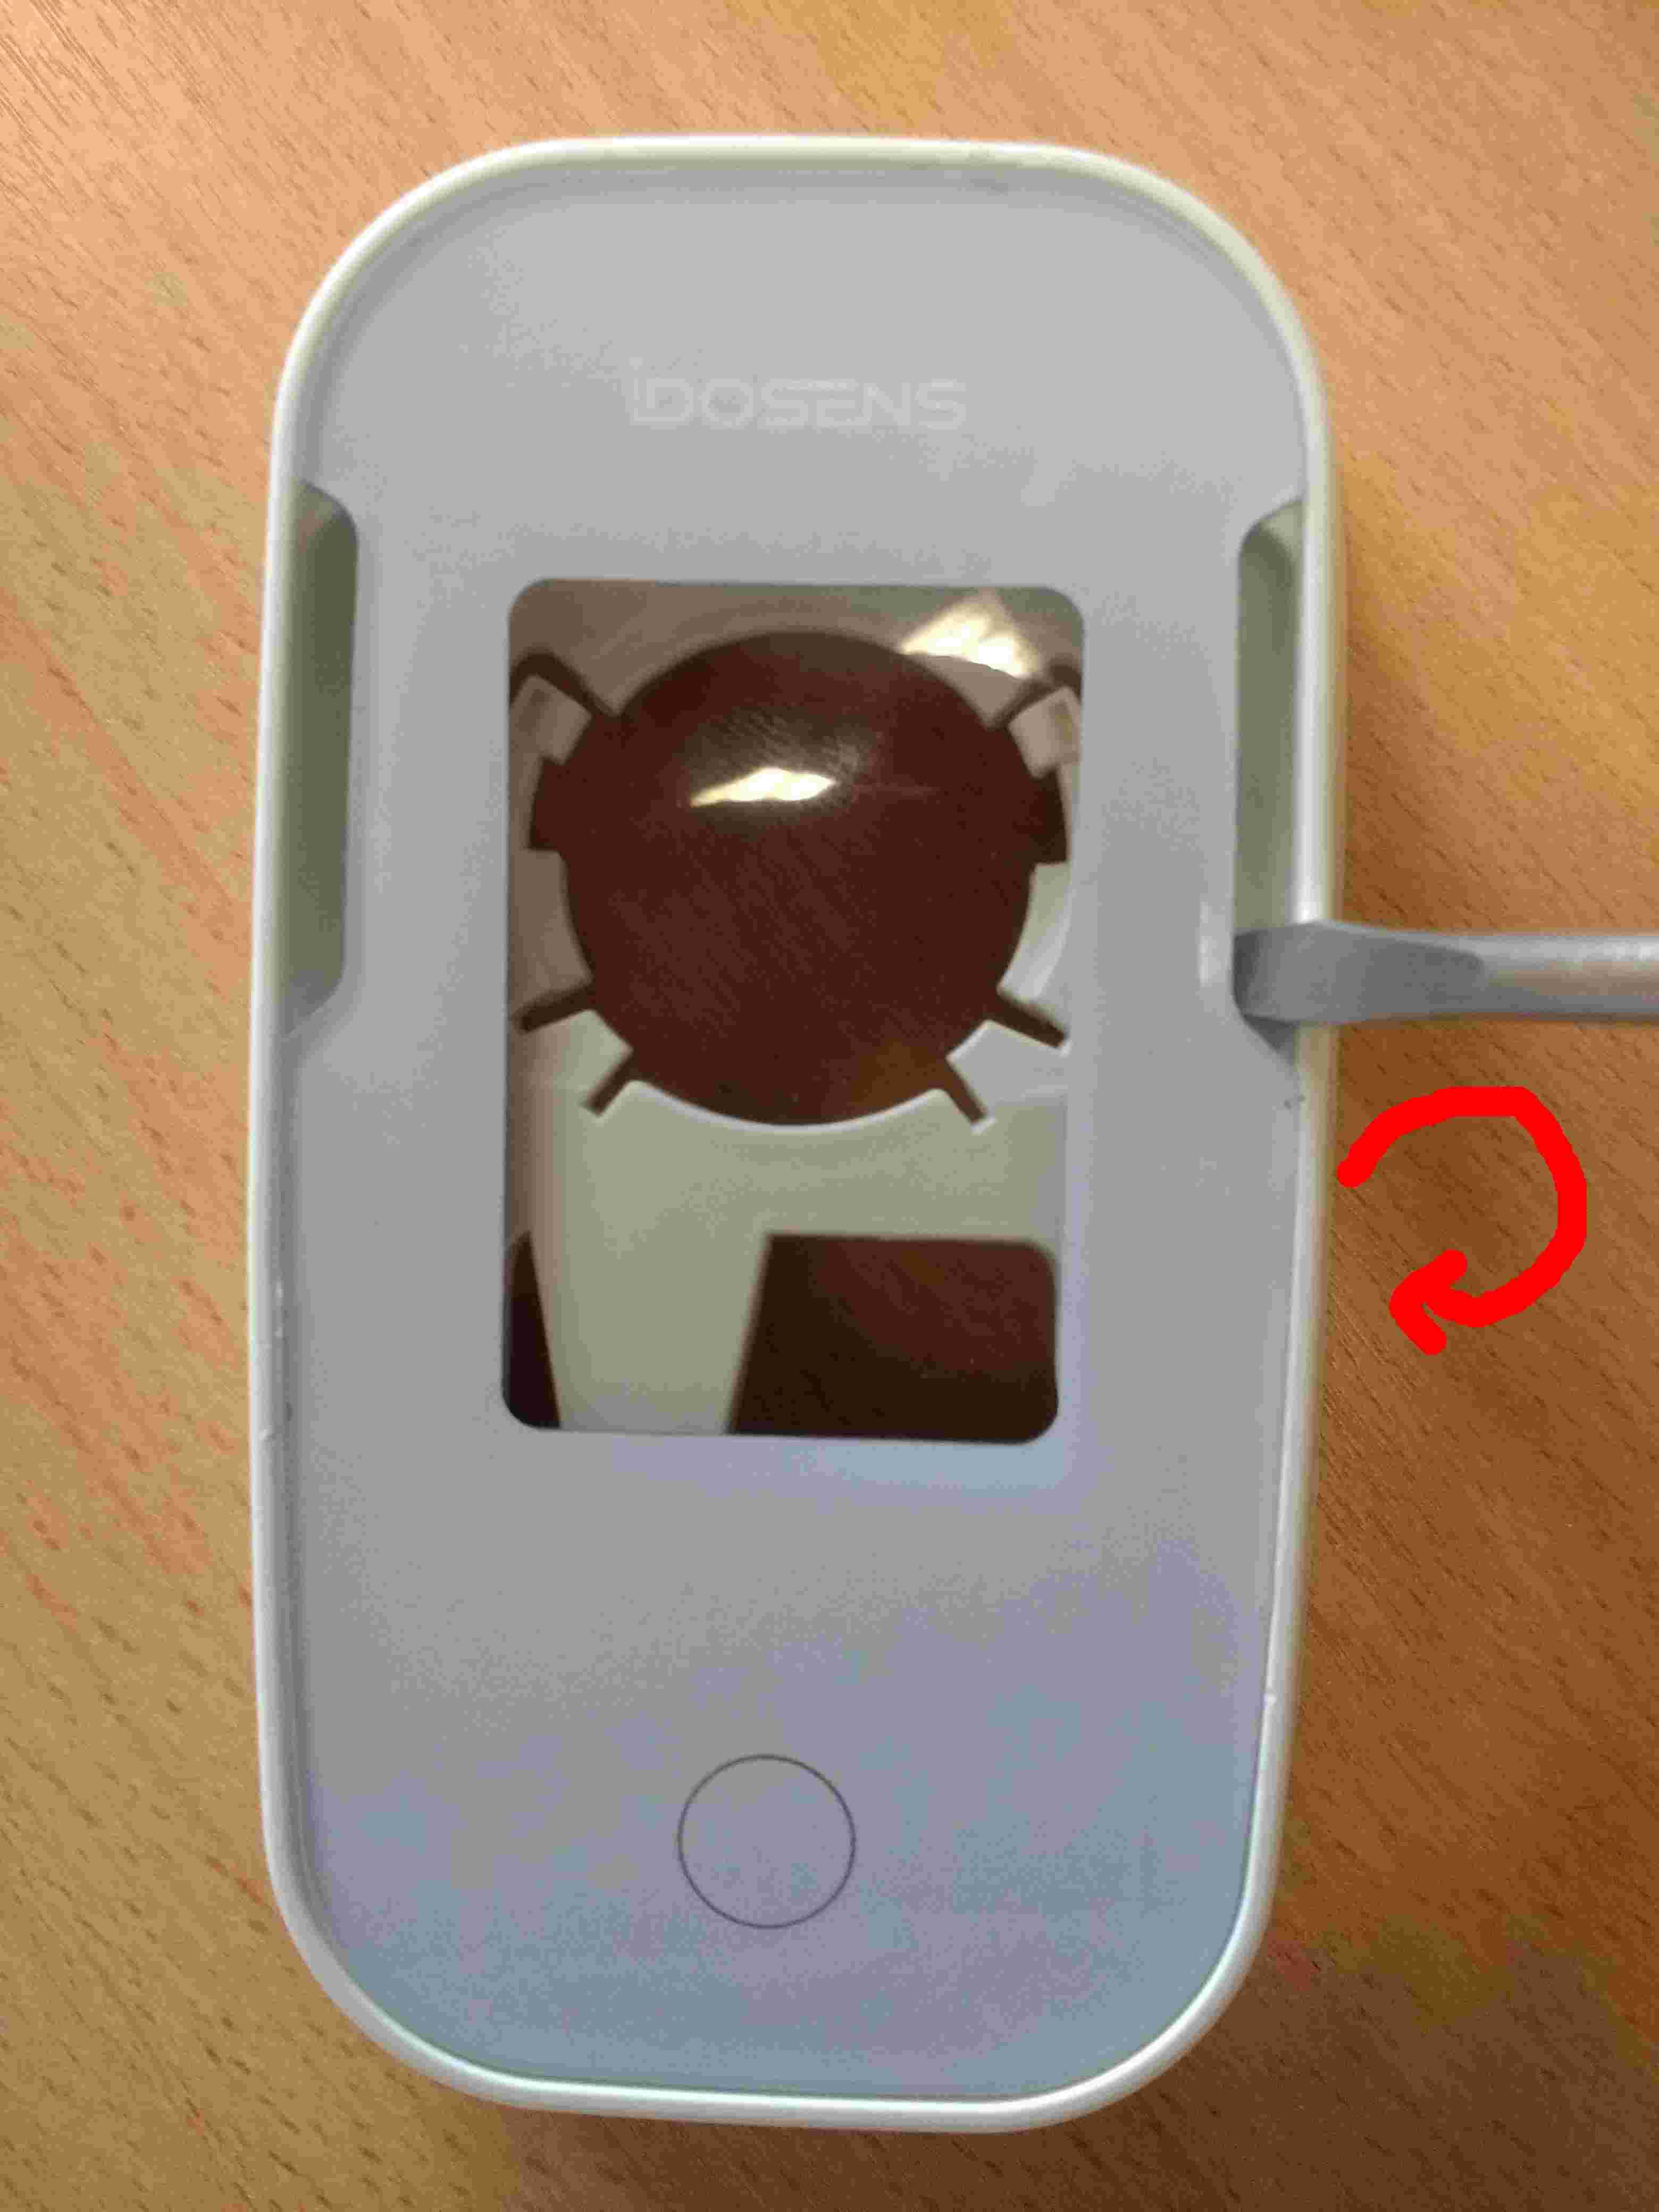
\includegraphics[keepaspectratio=true,scale=0.1]{enlever_ecran_idosens.jpg}
\label{visina8}
\end{center}\end{figure}

\begin{figure}[H]
\begin{center}
\advance\leftskip-3cm
\advance\rightskip-3cm
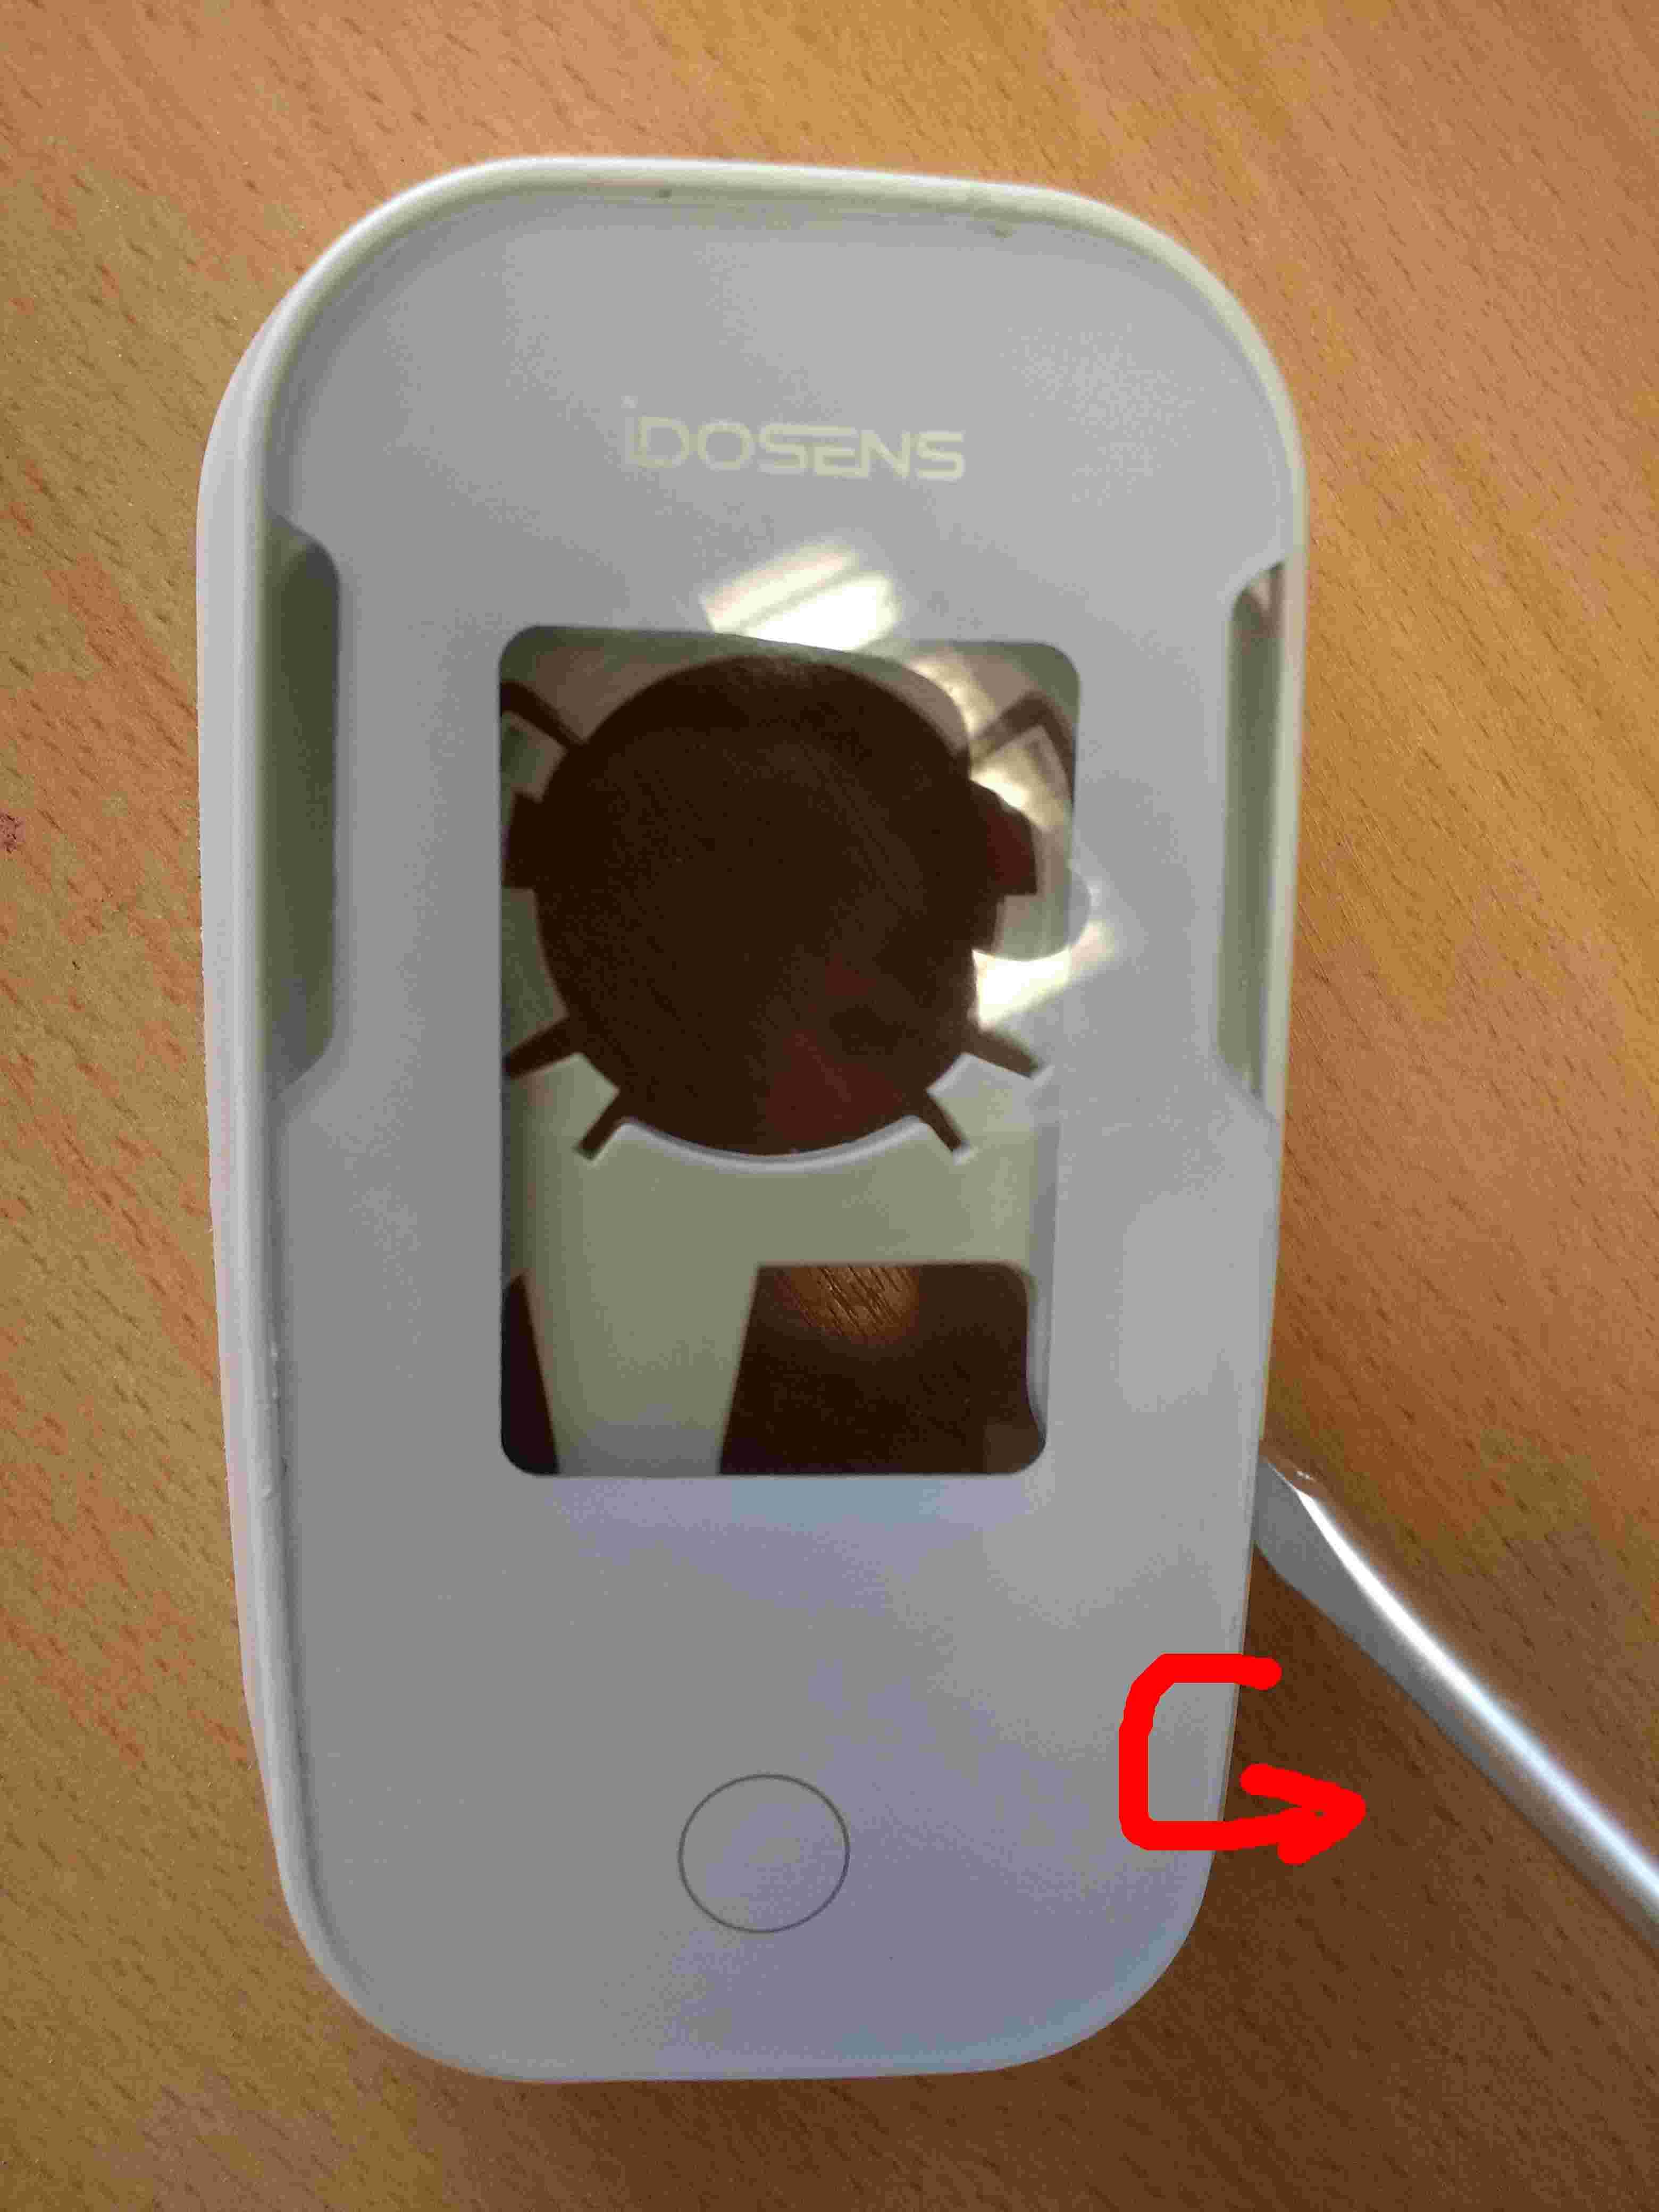
\includegraphics[keepaspectratio=true,scale=0.1]{remettre_ecran_idosens.jpg}
\label{visina8}
\end{center}\end{figure}

\end{document}
